\section{Boosting VoD delivery: The WiseReplica Approach}
\label{sec:replication_scheme}

In this section, we describe WiseReplica replication scheme. First, we highlight how WiseReplica operates in edge networks, by in introducing the concept of storage domains. Then, we explain its replication strategy based on predictions of ranking of video demand.

\subsection{Distributing VoD with Storage Domains}
\label{subsec:replication_scheme_sd}

% We evaluated this work with an implementation on top of PeerSim. We developed a tool which models a content distribution system for edge networks. 

We assume that WiseReplica operates in peer-assisted VoD systems deployed on hybrid CDN platforms. We consider the hybrid CDN design called Caju, that is detailed in our previous work~\cite{caju_tr_2012} as our target platform. It is based on sets of devices located close to customers, named storage domain. A storage domain is a logical
entity that combines resources from both datacenters and edge networks in the last mile of the content delivery chain. As Figure~\ref{fig:storage_domain} shows, devices in a storage domain can play either a coordinator or peer role. 

\noindent
\textbf{Coordinator} is a server or a small-sized cluster of servers deployed in the nearby datacenter. We assume that the coordinator performs scheduling of video requests for the local storage domains. Therefore, it runs the main instance of WiseReplica, and keeps information about resources consumption. Its main goal is to maintain the right number of replicas per video in the local peers, by pre-fetching or deleting sources. Instead of always contacting the content providers, coordinators might interoperate in logically centralized way to fetch videos that have been vanished from a storage domain. They store the most recent videos in their own cache for replication purposes. Whenever a new replica is necessary, the coordinator pushes it to a randomly, uniformly selected peer. Similarly, coordinators send video deletion requests to local peers. 

\noindent
\textbf{Peers} is a set of devices located close to each other through which customers get network access, e.g. home gateways connected to the same digital subscriber line access multiplexer (DSLAM). These devices actually deliver videos to customers in a storage domain, being the main source of storage and network resources. They execute scheduling and replication commands sent by the storage domain's coordinator. Each peer contributes with a percentage of storage and network resources to the system, as in a collaborative caching. In the local cache is applied the LRU policy for videos replacement.

This model is specially interesting for the problem of videos delivery as it takes advantage of nodes geographical position~\cite{Brodersen_www_2012}. It provides two main infrastructure properties to WiseReplica: replication group and hop limit.  The replication group allows WiseReplica to adapt video replication for smaller sets of peers, most likely connecting customers with similar content interests. By enforcing a hop limit, storage domains avoid jitter, ensure low latencies, and permit WiseReplica improving  the efficiency of network resource provision. 

In addition, we assume that a storage domain enforces an initial placement policy. This policy defines the minimum replication degree $m$ for initial copies for any new, just fetched Internet video.  Request scheduling is simple. A view request is served by at most $R$ nodes with uniform load. Available sources come from $r=min(n,R)$, where $n$ is the number of current replicas. In this work, we consider $m$ equals to two and $R$ equals to five as default settings. For requests scheduling, this approach enforces well-known policies for peers in edge networks, including nearest source selection and multi-sourcing. 


\begin{figure}[htbp]
  \centering
  \begin{minipage}[t]{1\linewidth}
    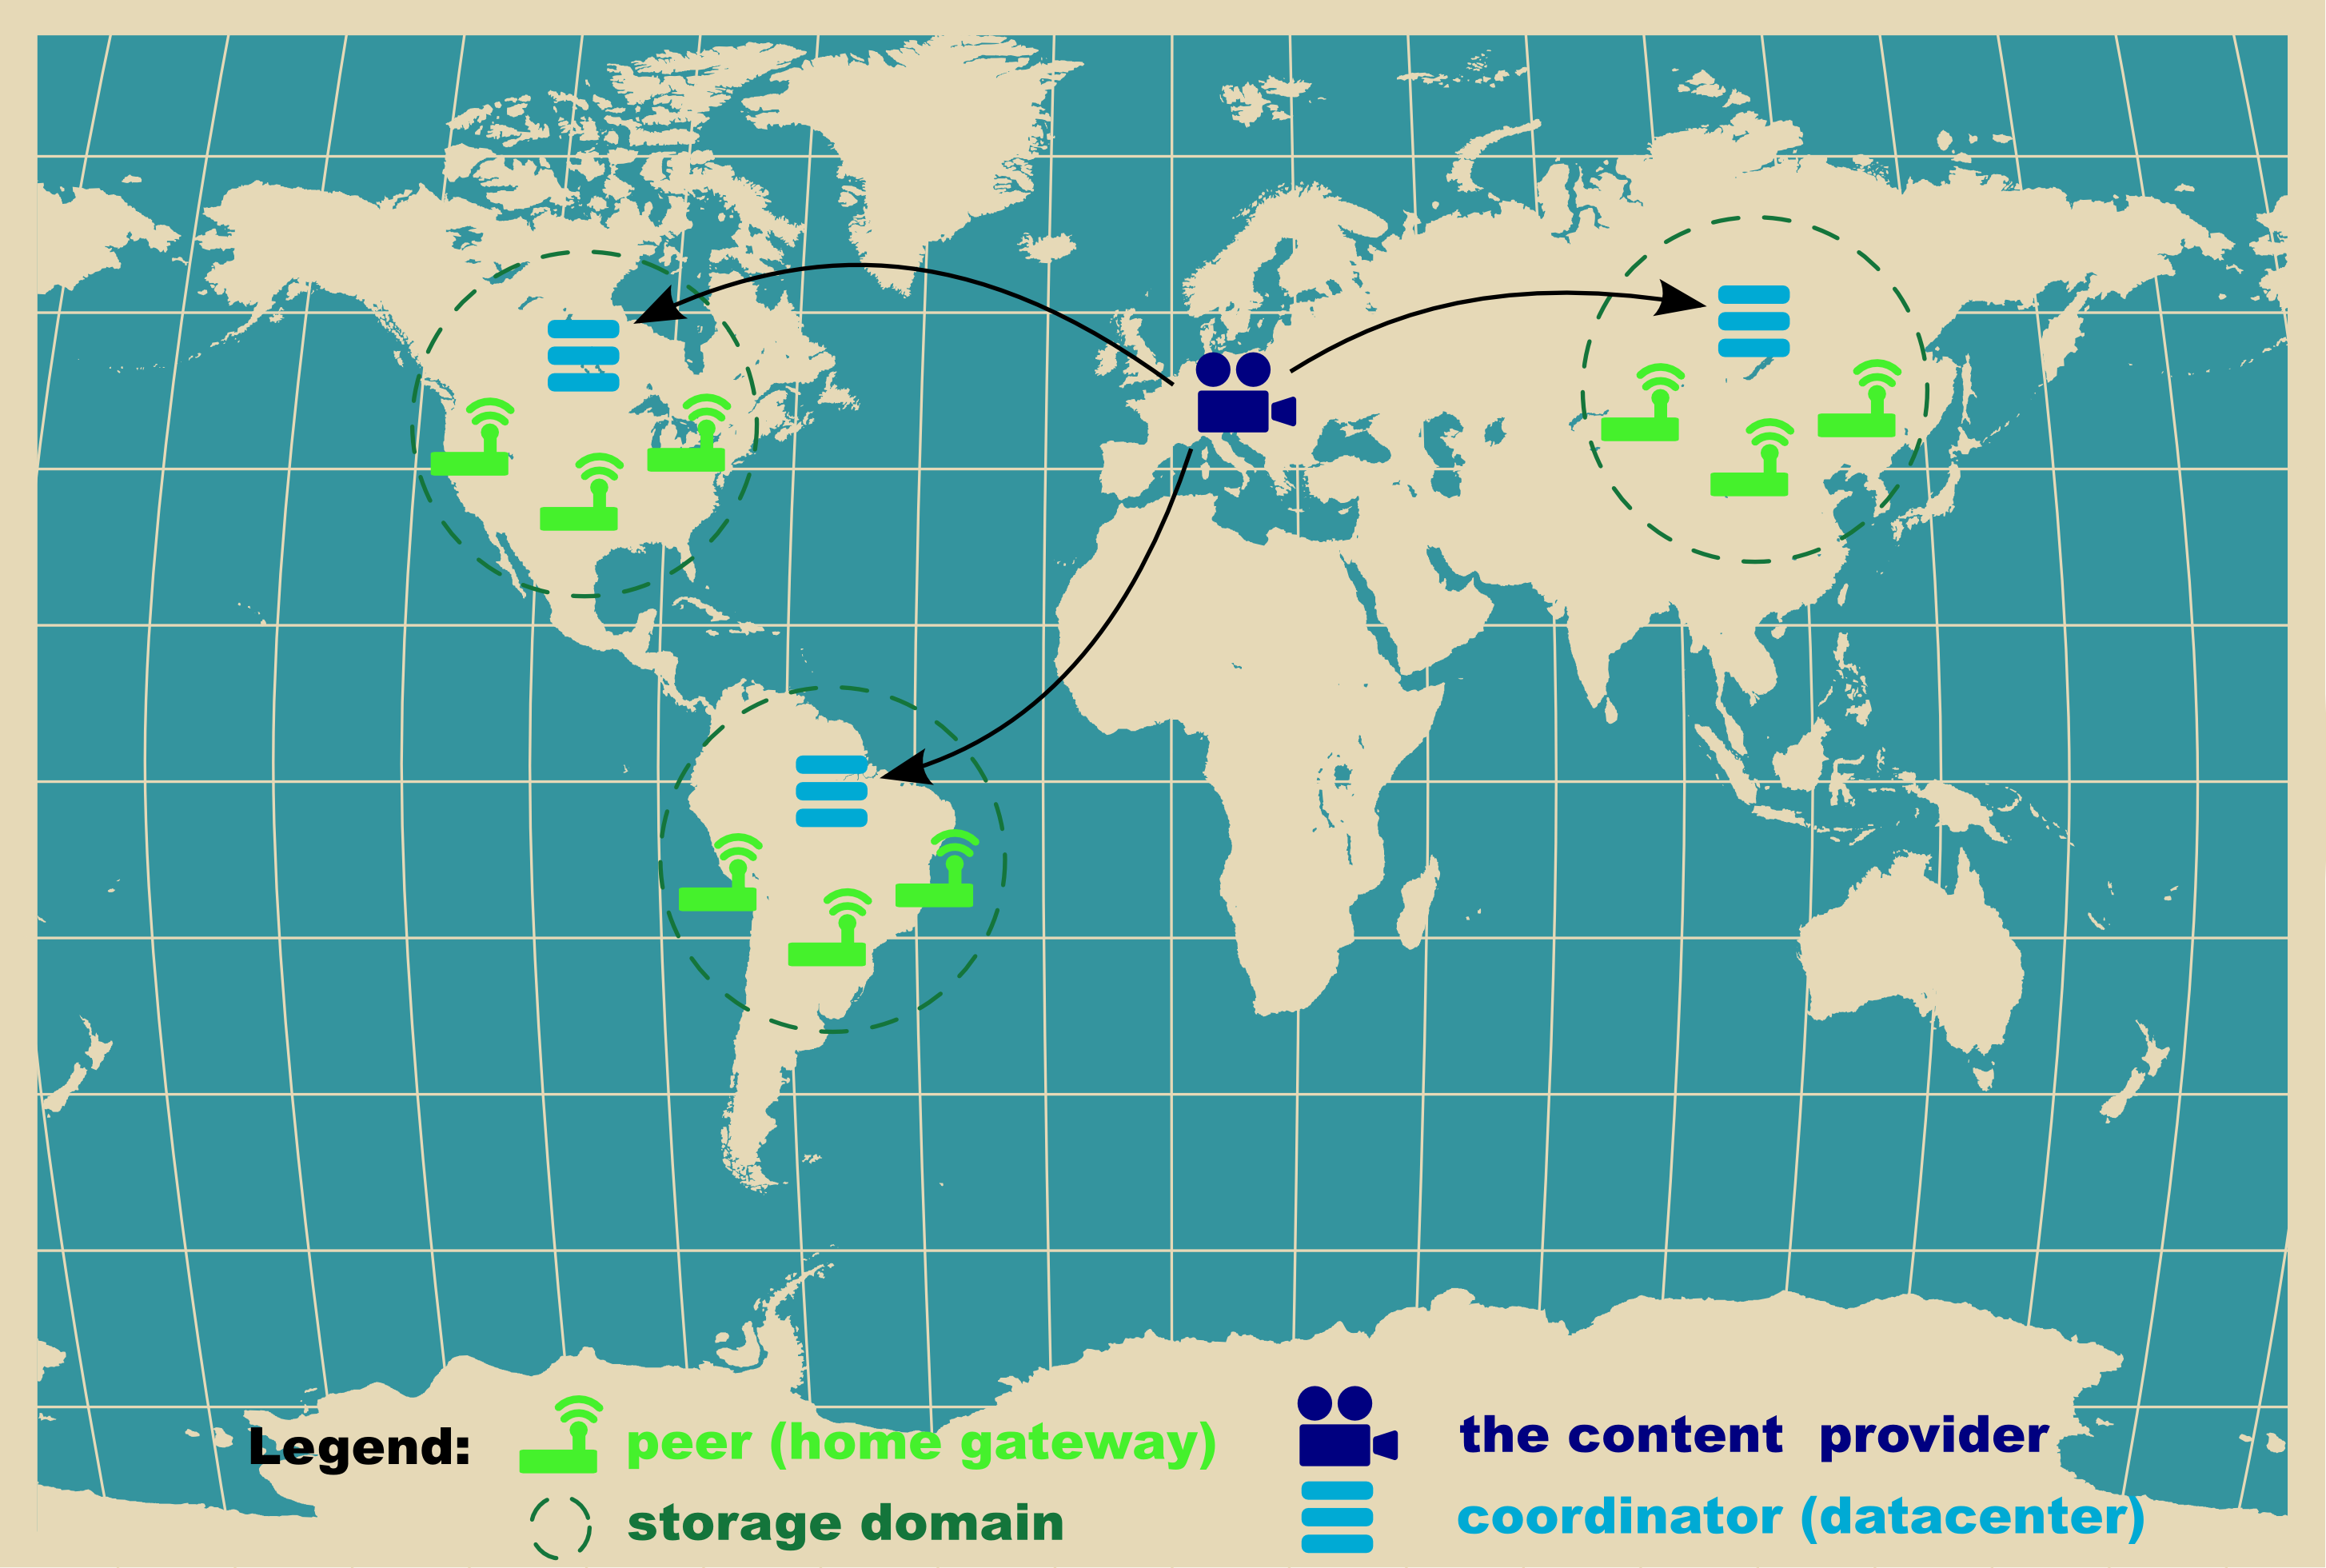
\includegraphics[width=1\textwidth]{inputs/img/sd}
    \caption{Storage domains.}
    \label{fig:storage_domain}
  \end{minipage}
\end{figure}

%We assume that the service provider infrastructure is organized in
%federated storage domains. A storage domain is a logical entity that
%aggregates a set of storage elements that are located close to each
%other, e.g. connected to a digital subscriber line access multiplexer
%(DSLAM). The storage elements are partitioned in two different
%classes: (i) operator-edge elements, furnished by storage operators,
%e.g. small-sized datacenters, and (ii) consumer-edge entities provided by
%consumers, such as set-top boxes. Consumer-edge devices contribute to
%storage and network resources according to their availability and
%load. Operator-edge nodes run a distributed storage system for local-area
%network over commodity servers. They provide cheap and high available
%resources dedicated to the storage service.
%
%On top of each Storage Domain runs a couple of services that deals with
%serving clients' requests, and performs appropriate object data
%placement and replication. 



\subsection{Self-adapting Replication According to the Ranking of Internet Videos}
\label{subsec:wisereplica_replication_strategy}

Our utmost goal is to contribute to meet increasing customers expectation on Internet videos using peer-assisted VoD systems. To enhance VoD delivery, we assume that rebuffering is a major issue to be addressed. We propose to cope with this issue by enforcing minimum average bitrate of each streaming as the main QoS metric. In this scenario, content and CDN providers must be committed to enforce minimum average bitrate for videos through SLA contracts. Since Internet videos delivery is a resource-hungry service, we must also adapt the network provision and storage usage as we aim to prevent violations. To this end, we propose WiseReplica, an adaptive replication scheme for peer-assisted VoD systems based on storage domains.

WiseReplica maintains replicas inside a storage domain. Running on the coordinator, it adapts the replication degree of Internet videos of a storage domain according to a machine-learned ranking. Our scheme follows a three-part procedure: 

\noindent
\textbf{Collect information from the request arrival process}. For each video request, WiseReplica collects 10 lightweight measurements. The goal is to gather comprehensive information for measuring the video demand and accurately predicting the raking. As described in Section~\ref{sec:learning_model}, they are video size, network availability, network usage (load), current number of viewers and replicas, inter-arrival time between requests (delta), aggregate number of views, mean of time between requests (mtbr), life time, and average bitrate. We compute averages and means from the last up to five requests. It is important to notice that all these measurements can be easily collected in the storage domain's coordinator.
 
\noindent
\textbf{Rank Internet videos in order of demand}. Based on the measurements of the request arrival process, we use the learning model described in Section~\ref{sec:learning_model} for predicting the rank position of Internet videos demand. We can predict the video rank for each view from the second request. The ranking comprises information about demand and QoS requirements. Predictions are quite essential for enhancing VoD delivery. Since our learning model make predictions on a request basis, WiseReplica can react to the video demand as promptly as the rank position evolves. Indeed, ranking is an intuitive way to capture the demand of videos in peer-assisted VoD systems. The higher is the demand rank position of an Internet video, the higher is the demand for it. There are four positions on our machine-learned ranking: \emph{non-popular, popular, very popular,} and \emph{viral}. WiseReplica has a straightforward strategy to perform replication according to hotness rank positions. Videos that fall into the lowest rank position can have their replication degree reduced, otherwise they need more replicas. Thus, the maintenance of replication degree of Internet video, including video creations and deletions in peers, relies on replication policies.

\noindent
\textbf{Enforce replication policy accordingly and in time}. The goal of replication policies is two-fold: first (i) ensure consumers' expectations in time and (ii) reduce the total number of replicas as much as possible. For that, WiseReplica must adapt replication of videos according to the forecasts of their rank positions. Our replication scheme enforces two types of replica maintenance policies: deletion and creation policy. In this work, we enforce a single video deletion policy.  Whenever the coordinator receives a request to a video in the non-popular rank, the deletion policy says that one replica is deleted until the minimum replication degree $m$ is reached. Similarly, our scheme periodically runs a maintenance procedure (e.g. each five minutes) to smoothly enforce the deletion policy for inactive videos. This allows WiseReplica to reduce the total number of replicas. To cope with SLA violations and meet customers' expectations, we evaluate four quite simple policies, namely uniform, linear, quadratic, and exponential. They are respectively defined as follows: $B$, $Br$,$Br^2$, and $B^r$, where $B$ is a constant that represents the target number of replicas, and $r \in \{1,2,3\}$ the rank positions. We report on creation policies' performances in Section~\ref{sec:evaluation}.


Our findings show that this approach produces a good balance between resource usage and consumers' satisfaction. It is important to note, however, WideReplica does not cover video durability, neither does fault-tolerant mechanisms (e.g. failure detection/recovery procedures). Rather, our goal is to improve VoD availability, boosting network provision, meeting consumers' expectations on VoD services, and reducing storage usage as much as possible. To this end, WiseReplica combines lightweight measurements, accurate predictions of Internet videos ranking, and replication policies enforcement in a particularly novel, flexible way. In peer-assisted VoD systems, it can easily interoperate with de facto approaches, including HTTP adaptive streaming technique and swarming protocols, such as BitTorrent. 
